\documentclass{beamer}
\usetheme{Boadilla}
\usepackage{booktabs}
\usepackage{adjustbox}
\usefonttheme{serif}
\subtitle{Using Beamer}
\usepackage{pgffor}

\title{ \textbf{Stepscan Project}}
\subtitle{Results of Worksheet 1-3}
\date{\today}
\author{Saeed Kazemi}
\institute{ University of New Brunswick}
\usepackage{caption}

\begin{document}


%%%%%%%%%%%%%%%%%%%%%%%%%%%%%%%%%%%%%%%%%%%
%%%%%%%%%%%%%%%%%%%%%%%%%%%%%%%%%%%%%%%%%%%
\begin{frame}
\titlepage
\end{frame}


%%%%%%%%%%%%%%%%%%%%%%%%%%%%%%%%%%%%%%%%%%%
%%%%%%%%%%%%%%%%%%%%%%%%%%%%%%%%%%%%%%%%%%%
\begin{frame}
\frametitle{Outline}
\tableofcontents
\end{frame}


%%%%%%%%%%%%%%%%%%%%%%%%%%%%%%%%%%%%%%%%%%%
%%%%%%%%%%%%%%%%%%%%%%%%%%%%%%%%%%%%%%%%%%%
\section{Score Matrix}
\foreach \n in {afeatures\_simple, afeatures\_otsu, pfeatures, COAs\_otsu, COAs\_simple, COPs}{
\begin{frame}
\frametitle{Euclidean distance vs Correlation + \n-Mode-Acc}
\tiny
\begin{table}
\centering
\captionsetup{labelformat=empty}
\caption{\footnotesize The accuracy of Euclidean distance and Correlation on COP features.}
\begin{tabular}{lll}
\toprule
{} &                  Accuracy Left &                 Accuracy Right \\
\midrule
Euclidean distance &  72.21 +/- 3.14 (67.67, 76.92) &  71.90 +/- 2.42 (68.69, 75.94) \\
Correlation        &  66.51 +/- 2.51 (62.50, 71.25) &  66.28 +/- 2.40 (63.09, 70.89) \\
\bottomrule
\end{tabular}

\end{table}
\begin{table}
\centering
\captionsetup{labelformat=empty}
\caption{\footnotesize The ERR of different size of the test set.}
\label{tab:parameters condition}
\input{Manuscripts/src/tables/\n-Mode-EER}
\end{table}

\begin{block}{\small Conditions}
    \footnotesize These results are average over the results of below conditions: min, mean and median criteria, All PCs and 95\% variances, Min-Max and z-score algorithm. 
\end{block}

\end{frame}



\begin{frame}
\centering
\frametitle{Euclidean distance vs Correlation (ROC curve)}
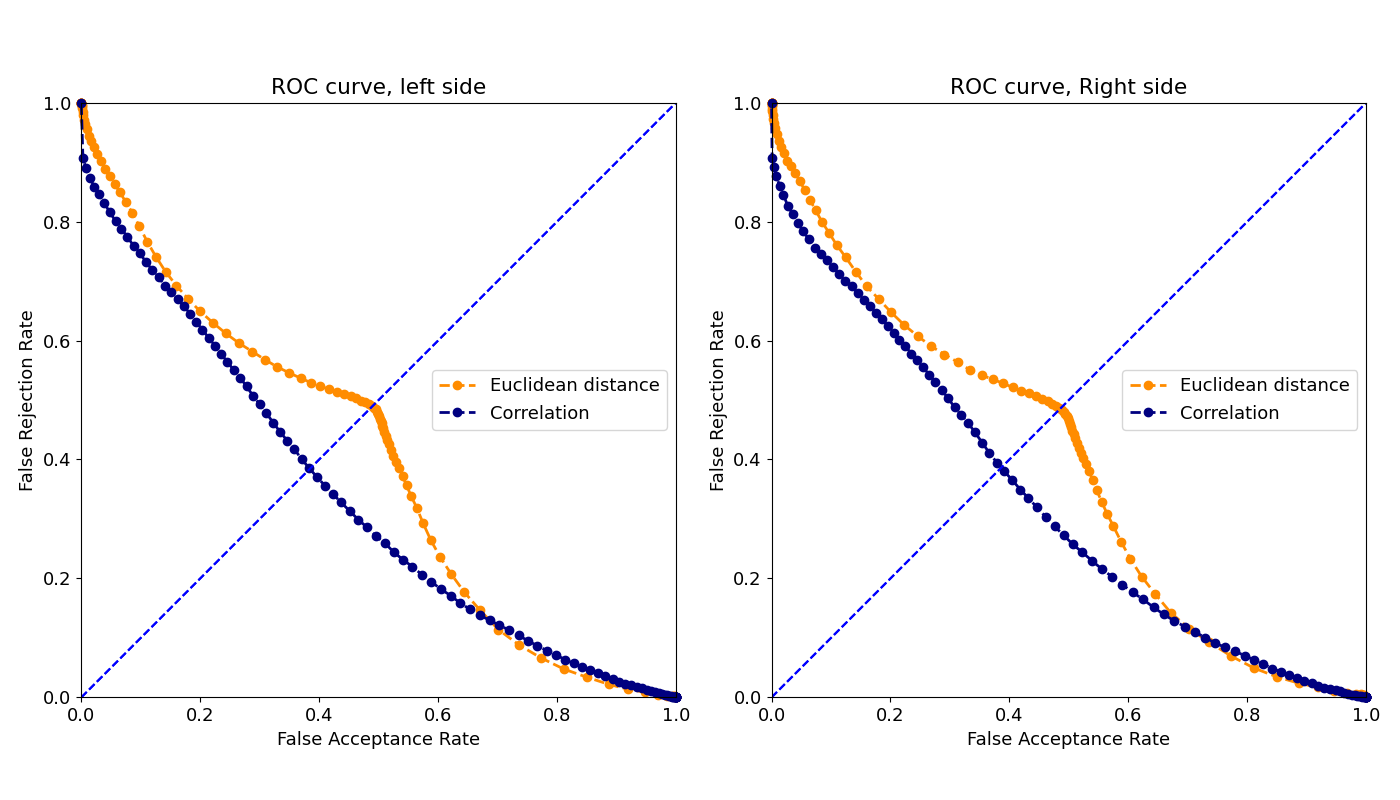
\includegraphics[scale=0.3]{Manuscripts/src/figures/pfeatures_Mode.png}
\end{frame}

}

\end{document}

